
\section{Background}
\label{sec:background}
While evolutionary algorithms have been used before to train and optimize neural networks these algorithms have not yet played a role in the efficient initialization and parameterization of neural networks. Efforts are largely focused on model architecture and training time for a single model. However, little work has been done concerning the specific initialization of a given model prior to training. Such initialization is usually performed randomly (i.e., the weights and biases of the model are initiated at a pseudo-random value). Following, it is possible, if not usual, when training a model multiple times, to arrive at very different results each time. This process of trial and error is repeated until an acceptable trained model is derived from some randomization. 
We therefore conceived that the purposeful selection of these initializations could allow for benefits in training a model and in merging partially trained models.

\begin{figure}[h!]
  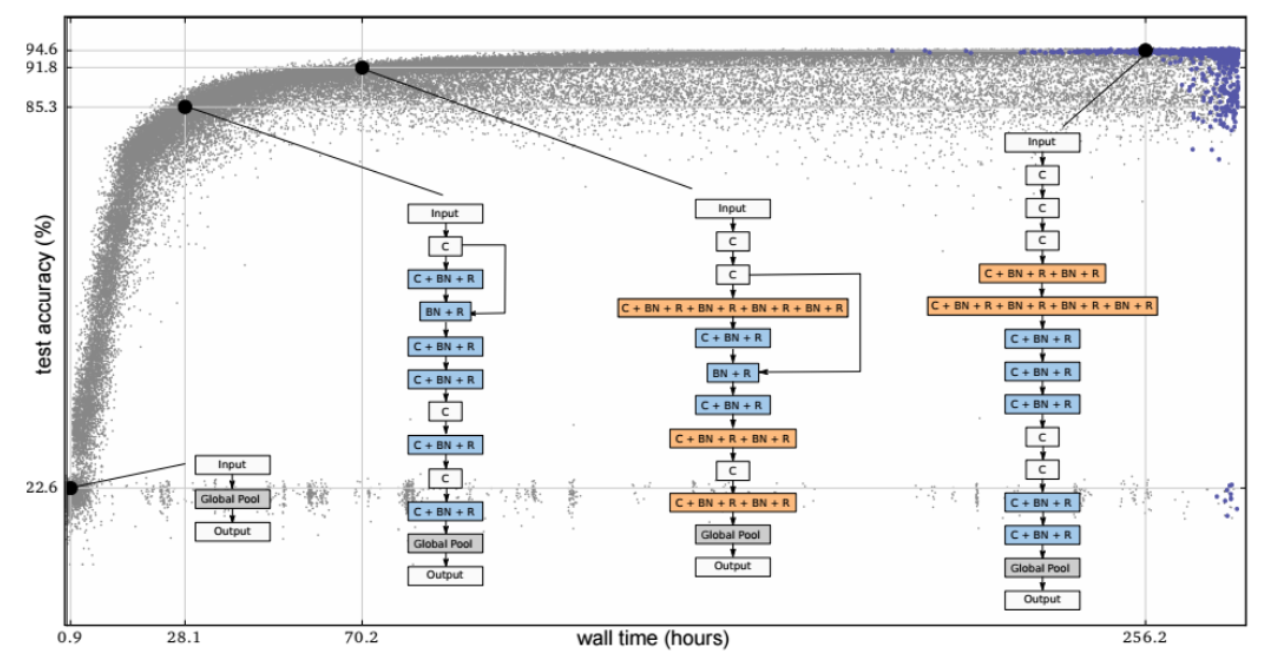
\includegraphics[width=\linewidth]{figures/nas.png}
  \caption{Neural architecture search become exponentially expensive with respect to marginal accuracy (Image credit: Towards Data Science, 2019)}
  \label{fig:nas}
\end{figure}




